\section{Ejercicio 1: Filtro anti-alias}
Se desea realizar un down-sampling de $f_s=10kHz$ a $f_s'=2kHz$. La señal de interés esta acotada en frecuencia hasta 970Hz; de este modo, con tal de evitar aliasing, se ha de diseñar un filtro pasa-bajos. 

En vista al problema planteado, se solicita que la atenuación en 970Hz resulte de 6dB y una atenuación de al menos 50dB a partir de $f_s'/2= 1000Hz$. 

\subsection{Diseño de filtro}
En función de los requerimientos previamente establecidos se diseña un filtro FIR mediante el método de la serie de Fourier. En este método resulta relevante la elección de la ventana a emplear en vista de optimizar el orden del filtro, donde varia, entre otras características, la atenuación del primer lóbulo lateral y la pendiente del lóbulo principal; afectando así el ancho de la banda de transición y la ganancia en la banda de atenuación. En vista a esta elección y en función de los requerimientos del filtro a implementar, se realizó una búsqueda entre las siguientes ventanas:

\begin{itemize}
    \item Rectangular.
    \item Bartlett.
    \item Hann.
    \item Hamming. 
    \item Blackman.
\end{itemize}

En función de este requerimiento, se implementó una búsqueda del número de taps necesario para cada una de ellas, con un máximo de 5000 (el proceso corresponde a buscar la función tal que la atenuación \underline{a partir} de $f_s'/2= 1000Hz$ sea de 50dB). Obteniendo así:

\vspace{1cm}
\begin{table}[H] 
\centering
\caption{Comparación de ventanas para el diseño del filtro FIR anti-alias}
\begin{tabular}{lccc}
\toprule
\textbf{Ventana} & \textbf{Orden mínimo (taps)} & \textbf{Atenuación mínima [dB]} & \textbf{Cumple} \\
\midrule
Rectangular (boxcar) & -- & -- & No \\
Bartlett             & -- & -- & No \\
Hann                 & 761 & 50.10 & Sí \\
Hamming              & 527 & 50.22 & Sí \\
Blackman             & 741 & 50.21 & Sí \\
\bottomrule
\end{tabular}
\label{tab: comparacion de ventanas}
\end{table}

\noindent donde además, se forzó en la búsqueda un número impar de taps tal que el filtro obtenido sea de fase lineal (por ende, group delay constante). 

En función de la tabla \ref{tab: comparacion de ventanas} se decide emplear la ventana de Hamming en el diseño del filtro. Bajo esta configuración se obtiene la siguiente respuesta en frecuencia:

\begin{figure}[H]
    \centering
    \begin{subfigure}{0.48\textwidth}
        \centering
        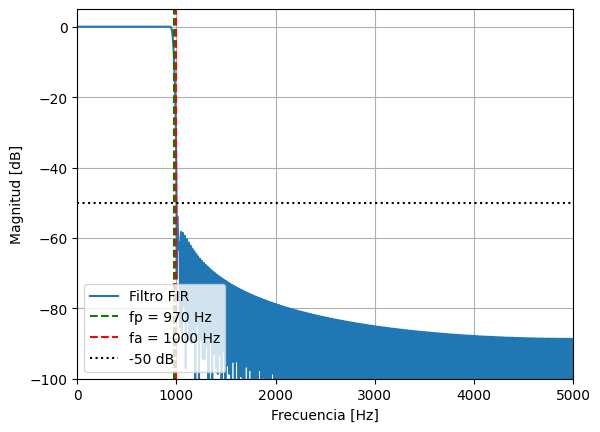
\includegraphics[width=\textwidth]{Imagenes/1_LPF_AL/rta_en_frec_ext.png}
        \caption{Extendida}
        \label{fig: magnitud rta en frec extendida}
    \end{subfigure}
    \hfill
    \begin{subfigure}{0.48\textwidth}
        \centering
        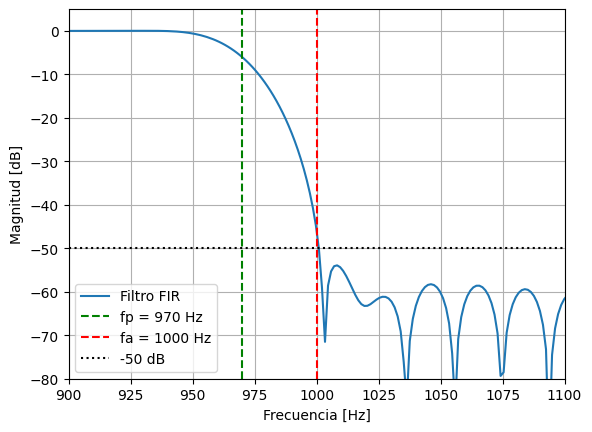
\includegraphics[width=\textwidth]{Imagenes/1_LPF_AL/rta_en_frec_det.png}
        \caption{Detalle}
        \label{fig: magnitud rta en frec extendida}
    \end{subfigure}
    \caption{Respuesta en frecuencia | Módulo}
    \label{fig: respuesta en frec_ mod}
\end{figure}


\noindent Donde se verifica el comportamiento esperado (no se muestra un detalle en las inmediaciones de 970Hz dado que la forma en la que se implemento garantiza la atenuación de 6dB allí).

En tanto a otras características fundamentales del filtro se puede analizar la fase:

\vspace{0.5cm}
\begin{figure}[H]
  \centering
  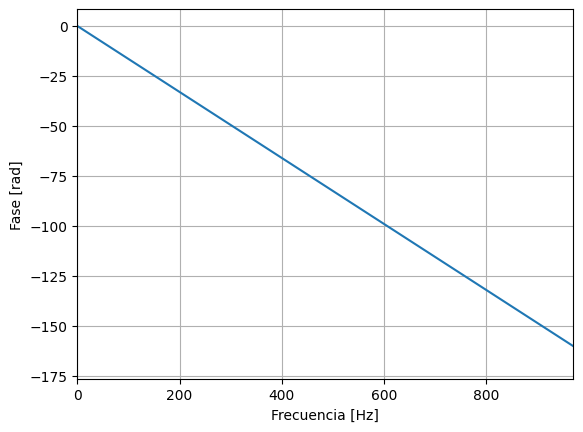
\includegraphics[width = 0.7 \textwidth]{Imagenes/1_LPF_AL/fase.png}
  \caption{Respuesta en frecuencia | Fase}
  \label{fig: rta en frec_fase}
\end{figure}

\noindent siendo relevante observar que efectivamente se dispone de fase lineal. Finalmente también resulta de interés observar la respuesta impulsiva del sistema:

\vspace{0.5cm}
\begin{figure}[H]
  \centering
  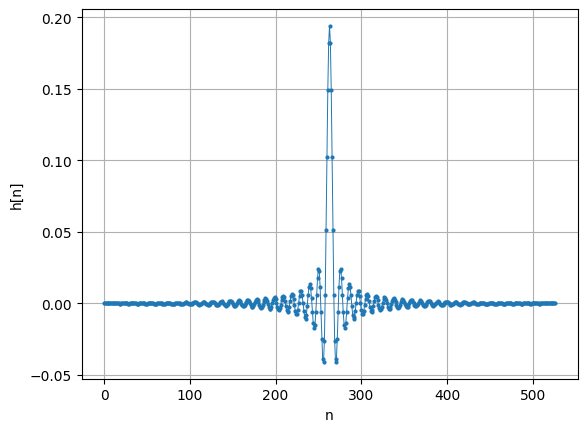
\includegraphics[width = 0.7 \textwidth]{Imagenes/1_LPF_AL/rta_al_escalon.png}
  \caption{Respuesta impulsiva.}
  \label{fig:  rta impulsiva}
\end{figure}

\noindent donde se observa la simetría para respecto a $N/2$.

\subsection{Implementación del sistema \& verificación empírica del funcionamiento}
Se realizó la implementación del filtro:

\vspace{0.5cm}
\begin{lstlisting}[style=mystyle, caption={Implementación del filtro.}, label={lst:filtro}]
def fir_filter(x, h):
    x = np.asarray(x)
    h = np.asarray(h)
    
    N = len(h)
    L = len(x)
    
    y = np.zeros(L)
    
    for n in range(L):
        for k in range(N):
            if n-k>=0:
                y[n] += h[k] * x[n-k]

    return y
\end{lstlisting}

\noindent tras la cual puede realizarse el down-sampling deseado:

\vspace{0.5cm}
\begin{lstlisting}[style=mystyle, caption={Filtrado + down-sampling.}, label={lst:filtro + ds}]
    # --- filtrado ---
    y = fir_filter(x, h)

    #--- down-sampling ---
    N_ds = 5

    y_ds = y[::N_ds]
    t_ds = t[::N_ds]
\end{lstlisting}


En el marco temporal, estas operaciones corresponden con las siguientes señales:

\begin{figure}[H]
    \centering
    \begin{subfigure}{0.48\textwidth}
        \centering
        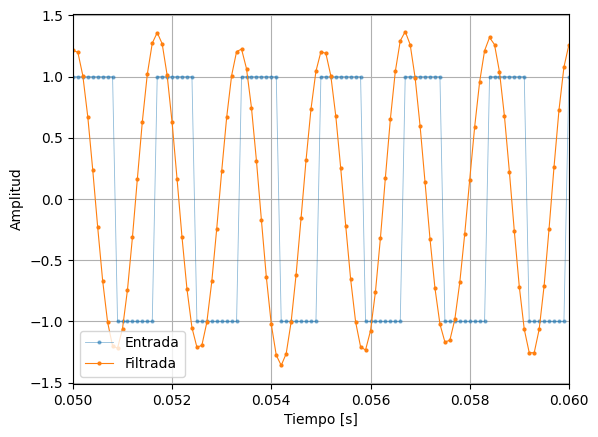
\includegraphics[width=\textwidth]{Imagenes/1_LPF_AL/filtrada_vs_sampled.png}
        \caption{Entrada + señal filtrada.}
        \label{fig: Entrada + señal filtrada.}
    \end{subfigure}
    \hfill
    \begin{subfigure}{0.48\textwidth}
        \centering
        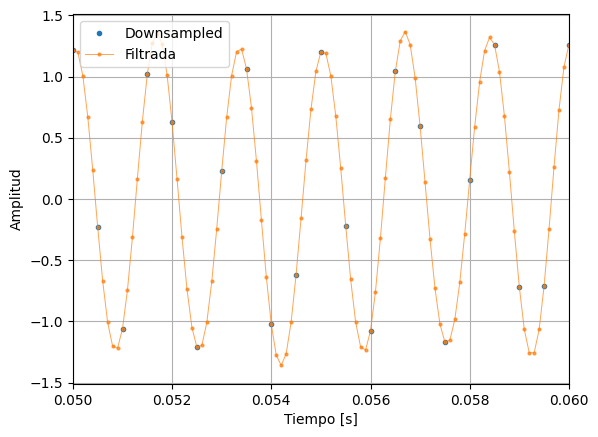
\includegraphics[width=\textwidth]{Imagenes/1_LPF_AL/filtrada_vs_down_sampled.png}
        \caption{Señal filtrada + downsampling.}
        \label{fig: Señal filtrada + downsampling.}
    \end{subfigure}
    \caption{Comparativa de señales en marco temporal}
    \label{fig: comparativa de seeñales en marco temporal}
\end{figure}

\noindent Esto se puede analizar desde el marco espectral realizando una FFT sobre las señales previamente indicadas:
\begin{figure}[H]
    \centering
    
    % --- fila superior ---
    \begin{subfigure}{0.48\textwidth}
        \centering
        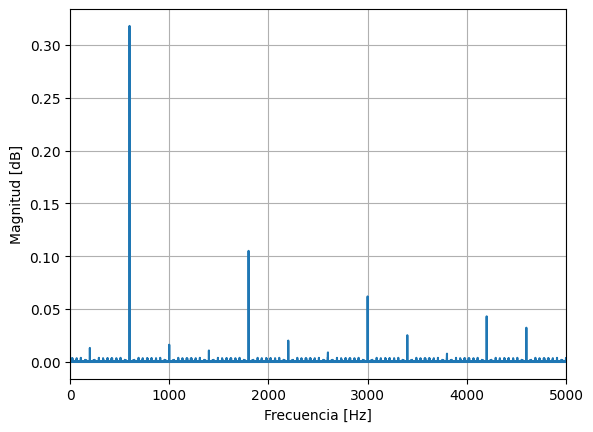
\includegraphics[width=\textwidth]{Imagenes/1_LPF_AL/entrada.png}
        \caption{Entrada}
    \end{subfigure}
    \hfill
    \begin{subfigure}{0.48\textwidth}
        \centering
        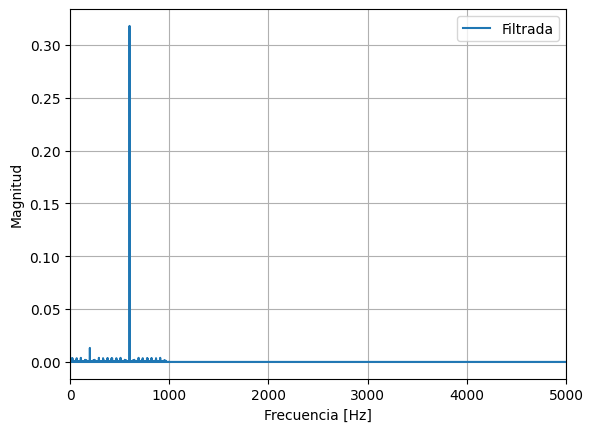
\includegraphics[width=\textwidth]{Imagenes/1_LPF_AL/filtrada_fft.png}
        \caption{Filtrada}
    \end{subfigure}

    \vspace{0.5cm}

    % --- fila inferior centrada ---
    \begin{subfigure}{0.48\textwidth}
        \centering
        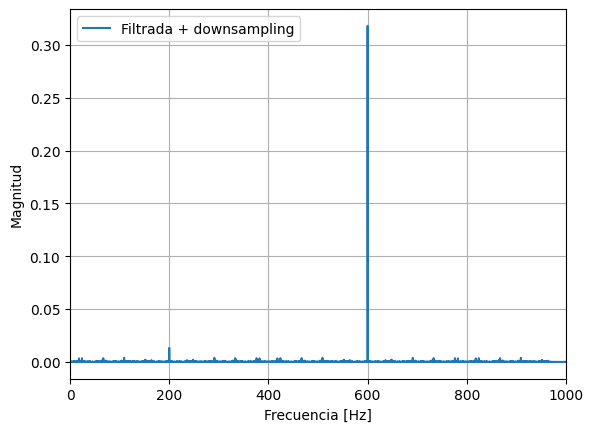
\includegraphics[width=\textwidth]{Imagenes/1_LPF_AL/filtrada_pls_ds_fft.png}
        \caption{Filtrada + down-sampling}
    \end{subfigure}

    \caption{Comparativa de señales en el dominio espectral}
\end{figure}

\noindent donde resulta relevante destacar que, por un lado, el cambio del rango en el eje corresponde a la modificación de la frecuencia de muestreo. Por otro lado, se observan armónicos que no eran esperados en función de la entrada indicada, estos se deben a que no se filtró la señal cuadrada a la hora de maestrearse, es decir, la entrada al sistema dispone de aliasing.

\subsection{Tiempo de procesamiento}
Se solicita calcular el tiempo de procesamiento del sistema. Para ello se realizaron 5 ejecuciones del código previamente indicado obteniendo:

\vspace{1cm}
\begin{table}[H] 
\centering
\caption{Tiempos de procesamiento del filtro FIR}
\begin{tabular}{lcc}
\toprule
\textbf{\#(Ejecución)} & \textbf{Tiempo [s]} & \textbf{Tiempo por muestra [$\mu$s]} \\
\midrule
1 & 19.135894 & 191.36 \\
2 & 18.456400 & 184.56 \\
3 & 18.152865 & 181.53 \\
4 & 18.438790 & 184.39 \\
5 & 18.219928 & 182.20 \\
\midrule
\textbf{Promedio} & 18.480776 & 184.808 \\
\bottomrule
\end{tabular}
\label{tab:tiempos_fir}
\end{table}
